\documentclass[twoside]{book}

% Packages required by doxygen
\usepackage{fixltx2e}
\usepackage{calc}
\usepackage{doxygen}
\usepackage[export]{adjustbox} % also loads graphicx
\usepackage{graphicx}
\usepackage[utf8]{inputenc}
\usepackage{makeidx}
\usepackage{multicol}
\usepackage{multirow}
\PassOptionsToPackage{warn}{textcomp}
\usepackage{textcomp}
\usepackage[nointegrals]{wasysym}
\usepackage[table]{xcolor}

% Font selection
\usepackage[T1]{fontenc}
\usepackage[scaled=.90]{helvet}
\usepackage{courier}
\usepackage{amssymb}
\usepackage{sectsty}
\renewcommand{\familydefault}{\sfdefault}
\allsectionsfont{%
  \fontseries{bc}\selectfont%
  \color{darkgray}%
}
\renewcommand{\DoxyLabelFont}{%
  \fontseries{bc}\selectfont%
  \color{darkgray}%
}
\newcommand{\+}{\discretionary{\mbox{\scriptsize$\hookleftarrow$}}{}{}}

% Page & text layout
\usepackage{geometry}
\geometry{%
  a4paper,%
  top=2.5cm,%
  bottom=2.5cm,%
  left=2.5cm,%
  right=2.5cm%
}
\tolerance=750
\hfuzz=15pt
\hbadness=750
\setlength{\emergencystretch}{15pt}
\setlength{\parindent}{0cm}
\setlength{\parskip}{3ex plus 2ex minus 2ex}
\makeatletter
\renewcommand{\paragraph}{%
  \@startsection{paragraph}{4}{0ex}{-1.0ex}{1.0ex}{%
    \normalfont\normalsize\bfseries\SS@parafont%
  }%
}
\renewcommand{\subparagraph}{%
  \@startsection{subparagraph}{5}{0ex}{-1.0ex}{1.0ex}{%
    \normalfont\normalsize\bfseries\SS@subparafont%
  }%
}
\makeatother

% Headers & footers
\usepackage{fancyhdr}
\pagestyle{fancyplain}
\fancyhead[LE]{\fancyplain{}{\bfseries\thepage}}
\fancyhead[CE]{\fancyplain{}{}}
\fancyhead[RE]{\fancyplain{}{\bfseries\leftmark}}
\fancyhead[LO]{\fancyplain{}{\bfseries\rightmark}}
\fancyhead[CO]{\fancyplain{}{}}
\fancyhead[RO]{\fancyplain{}{\bfseries\thepage}}
\fancyfoot[LE]{\fancyplain{}{}}
\fancyfoot[CE]{\fancyplain{}{}}
\fancyfoot[RE]{\fancyplain{}{\bfseries\scriptsize Generated by Doxygen }}
\fancyfoot[LO]{\fancyplain{}{\bfseries\scriptsize Generated by Doxygen }}
\fancyfoot[CO]{\fancyplain{}{}}
\fancyfoot[RO]{\fancyplain{}{}}
\renewcommand{\footrulewidth}{0.4pt}
\renewcommand{\chaptermark}[1]{%
  \markboth{#1}{}%
}
\renewcommand{\sectionmark}[1]{%
  \markright{\thesection\ #1}%
}

% Indices & bibliography
\usepackage{natbib}
\usepackage[titles]{tocloft}
\setcounter{tocdepth}{3}
\setcounter{secnumdepth}{5}
\makeindex

% Hyperlinks (required, but should be loaded last)
\usepackage{ifpdf}
\ifpdf
  \usepackage[pdftex,pagebackref=true]{hyperref}
\else
  \usepackage[ps2pdf,pagebackref=true]{hyperref}
\fi
\hypersetup{%
  colorlinks=true,%
  linkcolor=blue,%
  citecolor=blue,%
  unicode%
}

% Custom commands
\newcommand{\clearemptydoublepage}{%
  \newpage{\pagestyle{empty}\cleardoublepage}%
}

\usepackage{caption}
\captionsetup{labelsep=space,justification=centering,font={bf},singlelinecheck=off,skip=4pt,position=top}

%===== C O N T E N T S =====

\begin{document}

% Titlepage & ToC
\hypersetup{pageanchor=false,
             bookmarksnumbered=true,
             pdfencoding=unicode
            }
\pagenumbering{roman}
\begin{titlepage}
\vspace*{7cm}
\begin{center}%
{\Large pd2-\/\+Taiko }\\
\vspace*{1cm}
{\large Generated by Doxygen 1.8.11}\\
\end{center}
\end{titlepage}
\clearemptydoublepage
\tableofcontents
\clearemptydoublepage
\pagenumbering{arabic}
\hypersetup{pageanchor=true}

%--- Begin generated contents ---
\chapter{Namespace Index}
\section{Namespace List}
Here is a list of all namespaces with brief descriptions\+:\begin{DoxyCompactList}
\item\contentsline{section}{\hyperlink{namespaceUi}{Ui} }{\pageref{namespaceUi}}{}
\end{DoxyCompactList}

\chapter{Hierarchical Index}
\section{Class Hierarchy}
This inheritance list is sorted roughly, but not completely, alphabetically\+:\begin{DoxyCompactList}
\item Q\+Graphics\+Item\begin{DoxyCompactList}
\item \contentsline{section}{My\+Item}{\pageref{classMyItem}}{}
\item \contentsline{section}{My\+Item}{\pageref{classMyItem}}{}
\end{DoxyCompactList}
\item \contentsline{section}{qt\+\_\+meta\+\_\+stringdata\+\_\+\+Widget\+\_\+t}{\pageref{structqt__meta__stringdata__Widget__t}}{}
\item Q\+Widget\begin{DoxyCompactList}
\item \contentsline{section}{Widget}{\pageref{classWidget}}{}
\end{DoxyCompactList}
\item \contentsline{section}{Ui\+\_\+\+Widget}{\pageref{classUi__Widget}}{}
\begin{DoxyCompactList}
\item \contentsline{section}{Ui\+:\+:Widget}{\pageref{classUi_1_1Widget}}{}
\end{DoxyCompactList}
\end{DoxyCompactList}

\chapter{Class Index}
\section{Class List}
Here are the classes, structs, unions and interfaces with brief descriptions\+:\begin{DoxyCompactList}
\item\contentsline{section}{\hyperlink{class_my_item}{My\+Item} }{\pageref{class_my_item}}{}
\item\contentsline{section}{\hyperlink{class_widget}{Widget} }{\pageref{class_widget}}{}
\end{DoxyCompactList}

\chapter{File Index}
\section{File List}
Here is a list of all files with brief descriptions\+:\begin{DoxyCompactList}
\item\contentsline{section}{\hyperlink{main_8cpp}{main.\+cpp} }{\pageref{main_8cpp}}{}
\item\contentsline{section}{\hyperlink{myitem_8cpp}{myitem.\+cpp} }{\pageref{myitem_8cpp}}{}
\item\contentsline{section}{\hyperlink{myitem_8h}{myitem.\+h} }{\pageref{myitem_8h}}{}
\item\contentsline{section}{\hyperlink{widget_8cpp}{widget.\+cpp} }{\pageref{widget_8cpp}}{}
\item\contentsline{section}{\hyperlink{widget_8h}{widget.\+h} }{\pageref{widget_8h}}{}
\end{DoxyCompactList}

\chapter{Namespace Documentation}
\hypertarget{namespace_ui}{}\section{Ui Namespace Reference}
\label{namespace_ui}\index{Ui@{Ui}}

\chapter{Class Documentation}
\hypertarget{class_my_item}{}\section{My\+Item Class Reference}
\label{class_my_item}\index{My\+Item@{My\+Item}}


{\ttfamily \#include $<$myitem.\+h$>$}



Inheritance diagram for My\+Item\+:\nopagebreak
\begin{figure}[H]
\begin{center}
\leavevmode
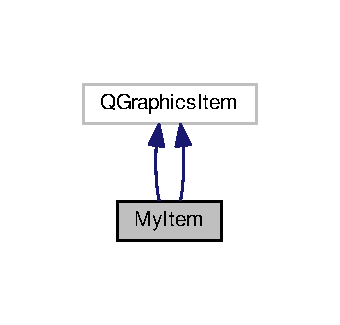
\includegraphics[width=163pt]{class_my_item__inherit__graph}
\end{center}
\end{figure}


Collaboration diagram for My\+Item\+:\nopagebreak
\begin{figure}[H]
\begin{center}
\leavevmode
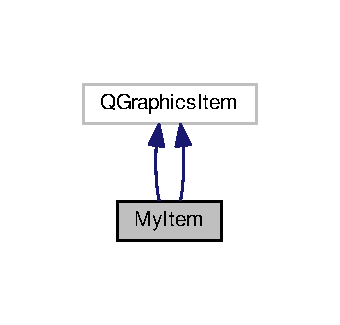
\includegraphics[width=163pt]{class_my_item__coll__graph}
\end{center}
\end{figure}
\subsection*{Public Member Functions}
\begin{DoxyCompactItemize}
\item 
\hyperlink{class_my_item_a9507a67820323a0c2fca0023aed44fed}{My\+Item} ()
\item 
Q\+RectF \hyperlink{class_my_item_ad287d7475bc642329fbc0e074bbe7458}{bounding\+Rect} () const 
\item 
void \hyperlink{class_my_item_ab038ec9fec1da2aba8fb9fa87d65b28d}{paint} (Q\+Painter $\ast$painter, const Q\+Style\+Option\+Graphics\+Item $\ast$option, Q\+Widget $\ast$widget)
\item 
\hyperlink{class_my_item_a9507a67820323a0c2fca0023aed44fed}{My\+Item} ()
\item 
Q\+RectF \hyperlink{class_my_item_ad287d7475bc642329fbc0e074bbe7458}{bounding\+Rect} () const 
\item 
void \hyperlink{class_my_item_ab038ec9fec1da2aba8fb9fa87d65b28d}{paint} (Q\+Painter $\ast$painter, const Q\+Style\+Option\+Graphics\+Item $\ast$option, Q\+Widget $\ast$widget)
\end{DoxyCompactItemize}
\subsection*{Public Attributes}
\begin{DoxyCompactItemize}
\item 
bool \hyperlink{class_my_item_a8062967505fab8ad3d54e71c04876c7f}{RG}
\item 
bool \hyperlink{class_my_item_aaeda1d0e2b67ff57fc2206c9e8d8e5e2}{valid}
\end{DoxyCompactItemize}
\subsection*{Protected Member Functions}
\begin{DoxyCompactItemize}
\item 
void \hyperlink{class_my_item_a0065ee31a5a17b10703e7edae0526814}{advance} (int phase)
\item 
void \hyperlink{class_my_item_a0065ee31a5a17b10703e7edae0526814}{advance} (int phase)
\end{DoxyCompactItemize}


\subsection{Detailed Description}


Definition at line 7 of file myitem.\+h.



\subsection{Constructor \& Destructor Documentation}
\index{My\+Item@{My\+Item}!My\+Item@{My\+Item}}
\index{My\+Item@{My\+Item}!My\+Item@{My\+Item}}
\subsubsection[{\texorpdfstring{My\+Item()}{MyItem()}}]{\setlength{\rightskip}{0pt plus 5cm}My\+Item\+::\+My\+Item (
\begin{DoxyParamCaption}
{}
\end{DoxyParamCaption}
)}\hypertarget{class_my_item_a9507a67820323a0c2fca0023aed44fed}{}\label{class_my_item_a9507a67820323a0c2fca0023aed44fed}


Definition at line 3 of file myitem.\+cpp.



Here is the caller graph for this function\+:
\nopagebreak
\begin{figure}[H]
\begin{center}
\leavevmode
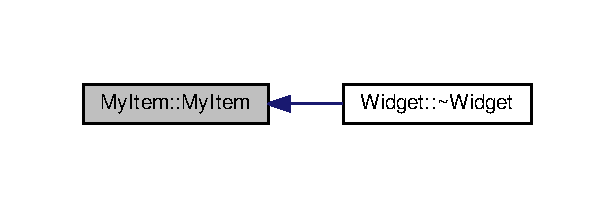
\includegraphics[width=295pt]{class_my_item_a9507a67820323a0c2fca0023aed44fed_icgraph}
\end{center}
\end{figure}


\index{My\+Item@{My\+Item}!My\+Item@{My\+Item}}
\index{My\+Item@{My\+Item}!My\+Item@{My\+Item}}
\subsubsection[{\texorpdfstring{My\+Item()}{MyItem()}}]{\setlength{\rightskip}{0pt plus 5cm}My\+Item\+::\+My\+Item (
\begin{DoxyParamCaption}
{}
\end{DoxyParamCaption}
)}\hypertarget{class_my_item_a9507a67820323a0c2fca0023aed44fed}{}\label{class_my_item_a9507a67820323a0c2fca0023aed44fed}


\subsection{Member Function Documentation}
\index{My\+Item@{My\+Item}!advance@{advance}}
\index{advance@{advance}!My\+Item@{My\+Item}}
\subsubsection[{\texorpdfstring{advance(int phase)}{advance(int phase)}}]{\setlength{\rightskip}{0pt plus 5cm}void My\+Item\+::advance (
\begin{DoxyParamCaption}
\item[{int}]{phase}
\end{DoxyParamCaption}
)\hspace{0.3cm}{\ttfamily [protected]}}\hypertarget{class_my_item_a0065ee31a5a17b10703e7edae0526814}{}\label{class_my_item_a0065ee31a5a17b10703e7edae0526814}


Definition at line 60 of file myitem.\+cpp.



Here is the call graph for this function\+:
\nopagebreak
\begin{figure}[H]
\begin{center}
\leavevmode
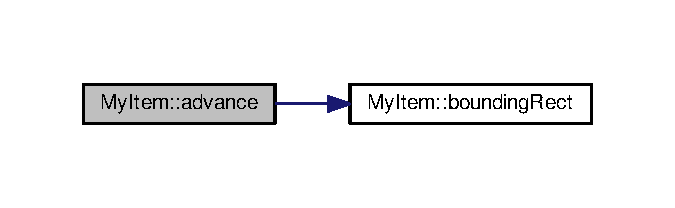
\includegraphics[width=324pt]{class_my_item_a0065ee31a5a17b10703e7edae0526814_cgraph}
\end{center}
\end{figure}




Here is the caller graph for this function\+:
\nopagebreak
\begin{figure}[H]
\begin{center}
\leavevmode
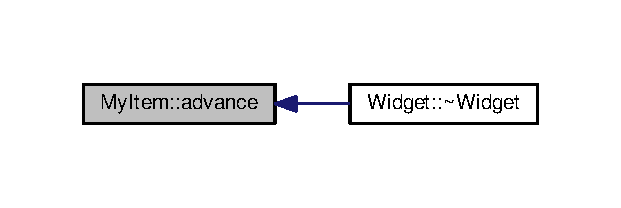
\includegraphics[width=298pt]{class_my_item_a0065ee31a5a17b10703e7edae0526814_icgraph}
\end{center}
\end{figure}


\index{My\+Item@{My\+Item}!advance@{advance}}
\index{advance@{advance}!My\+Item@{My\+Item}}
\subsubsection[{\texorpdfstring{advance(int phase)}{advance(int phase)}}]{\setlength{\rightskip}{0pt plus 5cm}void My\+Item\+::advance (
\begin{DoxyParamCaption}
\item[{int}]{phase}
\end{DoxyParamCaption}
)\hspace{0.3cm}{\ttfamily [protected]}}\hypertarget{class_my_item_a0065ee31a5a17b10703e7edae0526814}{}\label{class_my_item_a0065ee31a5a17b10703e7edae0526814}
\index{My\+Item@{My\+Item}!bounding\+Rect@{bounding\+Rect}}
\index{bounding\+Rect@{bounding\+Rect}!My\+Item@{My\+Item}}
\subsubsection[{\texorpdfstring{bounding\+Rect() const }{boundingRect() const }}]{\setlength{\rightskip}{0pt plus 5cm}Q\+RectF My\+Item\+::bounding\+Rect (
\begin{DoxyParamCaption}
{}
\end{DoxyParamCaption}
) const}\hypertarget{class_my_item_ad287d7475bc642329fbc0e074bbe7458}{}\label{class_my_item_ad287d7475bc642329fbc0e074bbe7458}


Definition at line 30 of file myitem.\+cpp.



Here is the caller graph for this function\+:
\nopagebreak
\begin{figure}[H]
\begin{center}
\leavevmode
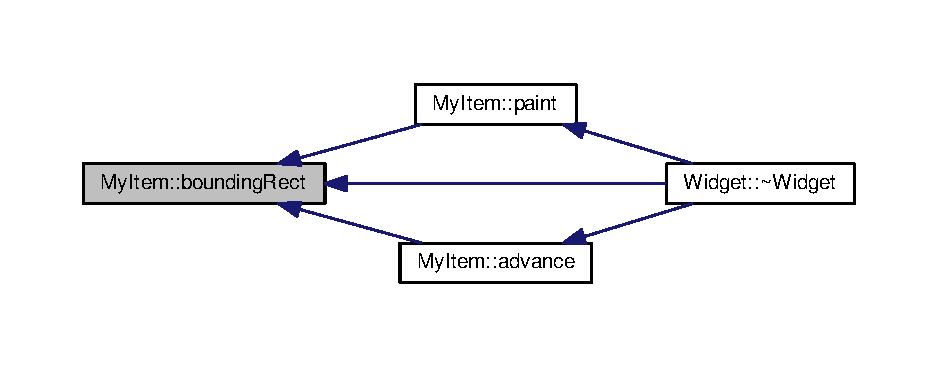
\includegraphics[width=350pt]{class_my_item_ad287d7475bc642329fbc0e074bbe7458_icgraph}
\end{center}
\end{figure}


\index{My\+Item@{My\+Item}!bounding\+Rect@{bounding\+Rect}}
\index{bounding\+Rect@{bounding\+Rect}!My\+Item@{My\+Item}}
\subsubsection[{\texorpdfstring{bounding\+Rect() const }{boundingRect() const }}]{\setlength{\rightskip}{0pt plus 5cm}Q\+RectF My\+Item\+::bounding\+Rect (
\begin{DoxyParamCaption}
{}
\end{DoxyParamCaption}
) const}\hypertarget{class_my_item_ad287d7475bc642329fbc0e074bbe7458}{}\label{class_my_item_ad287d7475bc642329fbc0e074bbe7458}
\index{My\+Item@{My\+Item}!paint@{paint}}
\index{paint@{paint}!My\+Item@{My\+Item}}
\subsubsection[{\texorpdfstring{paint(\+Q\+Painter $\ast$painter, const Q\+Style\+Option\+Graphics\+Item $\ast$option, Q\+Widget $\ast$widget)}{paint(QPainter *painter, const QStyleOptionGraphicsItem *option, QWidget *widget)}}]{\setlength{\rightskip}{0pt plus 5cm}void My\+Item\+::paint (
\begin{DoxyParamCaption}
\item[{Q\+Painter $\ast$}]{painter, }
\item[{const Q\+Style\+Option\+Graphics\+Item $\ast$}]{option, }
\item[{Q\+Widget $\ast$}]{widget}
\end{DoxyParamCaption}
)}\hypertarget{class_my_item_ab038ec9fec1da2aba8fb9fa87d65b28d}{}\label{class_my_item_ab038ec9fec1da2aba8fb9fa87d65b28d}


Definition at line 35 of file myitem.\+cpp.



Here is the call graph for this function\+:
\nopagebreak
\begin{figure}[H]
\begin{center}
\leavevmode
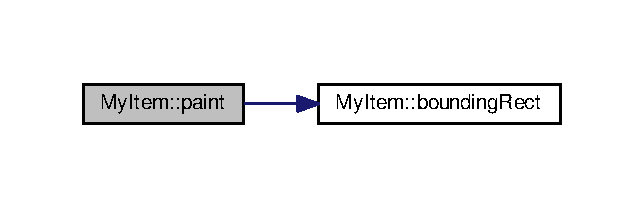
\includegraphics[width=309pt]{class_my_item_ab038ec9fec1da2aba8fb9fa87d65b28d_cgraph}
\end{center}
\end{figure}




Here is the caller graph for this function\+:
\nopagebreak
\begin{figure}[H]
\begin{center}
\leavevmode
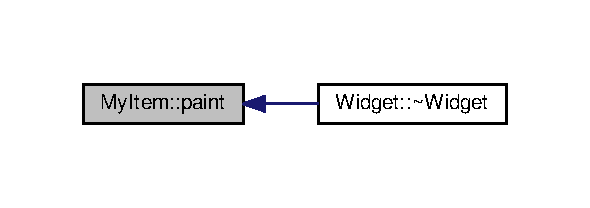
\includegraphics[width=283pt]{class_my_item_ab038ec9fec1da2aba8fb9fa87d65b28d_icgraph}
\end{center}
\end{figure}


\index{My\+Item@{My\+Item}!paint@{paint}}
\index{paint@{paint}!My\+Item@{My\+Item}}
\subsubsection[{\texorpdfstring{paint(\+Q\+Painter $\ast$painter, const Q\+Style\+Option\+Graphics\+Item $\ast$option, Q\+Widget $\ast$widget)}{paint(QPainter *painter, const QStyleOptionGraphicsItem *option, QWidget *widget)}}]{\setlength{\rightskip}{0pt plus 5cm}void My\+Item\+::paint (
\begin{DoxyParamCaption}
\item[{Q\+Painter $\ast$}]{painter, }
\item[{const Q\+Style\+Option\+Graphics\+Item $\ast$}]{option, }
\item[{Q\+Widget $\ast$}]{widget}
\end{DoxyParamCaption}
)}\hypertarget{class_my_item_ab038ec9fec1da2aba8fb9fa87d65b28d}{}\label{class_my_item_ab038ec9fec1da2aba8fb9fa87d65b28d}


\subsection{Member Data Documentation}
\index{My\+Item@{My\+Item}!RG@{RG}}
\index{RG@{RG}!My\+Item@{My\+Item}}
\subsubsection[{\texorpdfstring{RG}{RG}}]{\setlength{\rightskip}{0pt plus 5cm}bool My\+Item\+::\+RG}\hypertarget{class_my_item_a8062967505fab8ad3d54e71c04876c7f}{}\label{class_my_item_a8062967505fab8ad3d54e71c04876c7f}


Definition at line 68 of file widget.\+h.

\index{My\+Item@{My\+Item}!valid@{valid}}
\index{valid@{valid}!My\+Item@{My\+Item}}
\subsubsection[{\texorpdfstring{valid}{valid}}]{\setlength{\rightskip}{0pt plus 5cm}bool My\+Item\+::valid}\hypertarget{class_my_item_aaeda1d0e2b67ff57fc2206c9e8d8e5e2}{}\label{class_my_item_aaeda1d0e2b67ff57fc2206c9e8d8e5e2}


Definition at line 70 of file widget.\+h.



The documentation for this class was generated from the following files\+:\begin{DoxyCompactItemize}
\item 
\hyperlink{myitem_8h}{myitem.\+h}\item 
\hyperlink{widget_8h}{widget.\+h}\item 
\hyperlink{myitem_8cpp}{myitem.\+cpp}\item 
\hyperlink{widget_8cpp}{widget.\+cpp}\end{DoxyCompactItemize}

\hypertarget{class_widget}{}\section{Widget Class Reference}
\label{class_widget}\index{Widget@{Widget}}


{\ttfamily \#include $<$widget.\+h$>$}



Inheritance diagram for Widget\+:\nopagebreak
\begin{figure}[H]
\begin{center}
\leavevmode
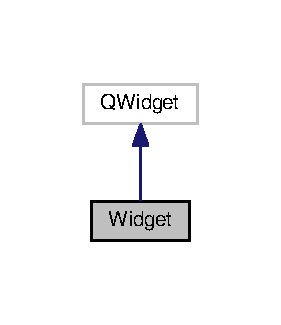
\includegraphics[width=135pt]{class_widget__inherit__graph}
\end{center}
\end{figure}


Collaboration diagram for Widget\+:\nopagebreak
\begin{figure}[H]
\begin{center}
\leavevmode
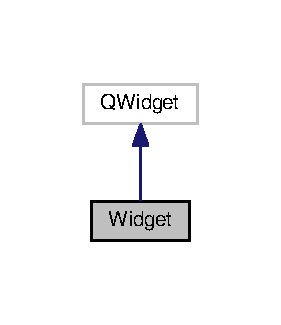
\includegraphics[width=135pt]{class_widget__coll__graph}
\end{center}
\end{figure}
\subsection*{Public Member Functions}
\begin{DoxyCompactItemize}
\item 
\hyperlink{class_widget_a29531c7f141e461322981b3b579d4590}{Widget} (Q\+Widget $\ast$parent=0)
\item 
\hyperlink{class_widget_aa24f66bcbaaec6d458b0980e8c8eae65}{$\sim$\+Widget} ()
\end{DoxyCompactItemize}
\subsection*{Protected Member Functions}
\begin{DoxyCompactItemize}
\item 
void \hyperlink{class_widget_a96b48889b8c1b29ecb2804008fbc89be}{key\+Press\+Event} (Q\+Key\+Event $\ast$e)
\end{DoxyCompactItemize}


\subsection{Detailed Description}


Definition at line 22 of file widget.\+h.



\subsection{Constructor \& Destructor Documentation}
\index{Widget@{Widget}!Widget@{Widget}}
\index{Widget@{Widget}!Widget@{Widget}}
\subsubsection[{\texorpdfstring{Widget(\+Q\+Widget $\ast$parent=0)}{Widget(QWidget *parent=0)}}]{\setlength{\rightskip}{0pt plus 5cm}Widget\+::\+Widget (
\begin{DoxyParamCaption}
\item[{Q\+Widget $\ast$}]{parent = {\ttfamily 0}}
\end{DoxyParamCaption}
)\hspace{0.3cm}{\ttfamily [explicit]}}\hypertarget{class_widget_a29531c7f141e461322981b3b579d4590}{}\label{class_widget_a29531c7f141e461322981b3b579d4590}


Definition at line 6 of file widget.\+cpp.

\index{Widget@{Widget}!````~Widget@{$\sim$\+Widget}}
\index{````~Widget@{$\sim$\+Widget}!Widget@{Widget}}
\subsubsection[{\texorpdfstring{$\sim$\+Widget()}{~Widget()}}]{\setlength{\rightskip}{0pt plus 5cm}Widget\+::$\sim$\+Widget (
\begin{DoxyParamCaption}
{}
\end{DoxyParamCaption}
)}\hypertarget{class_widget_aa24f66bcbaaec6d458b0980e8c8eae65}{}\label{class_widget_aa24f66bcbaaec6d458b0980e8c8eae65}


Definition at line 33 of file widget.\+cpp.



Here is the call graph for this function\+:
\nopagebreak
\begin{figure}[H]
\begin{center}
\leavevmode
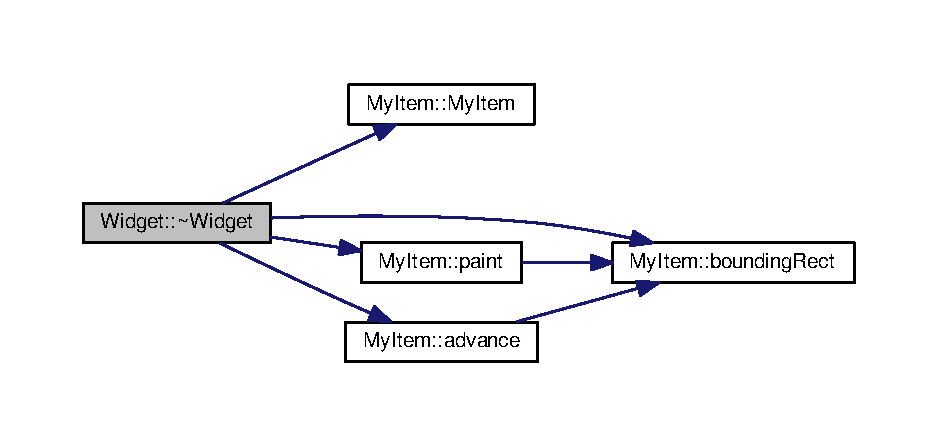
\includegraphics[width=350pt]{class_widget_aa24f66bcbaaec6d458b0980e8c8eae65_cgraph}
\end{center}
\end{figure}




\subsection{Member Function Documentation}
\index{Widget@{Widget}!key\+Press\+Event@{key\+Press\+Event}}
\index{key\+Press\+Event@{key\+Press\+Event}!Widget@{Widget}}
\subsubsection[{\texorpdfstring{key\+Press\+Event(\+Q\+Key\+Event $\ast$e)}{keyPressEvent(QKeyEvent *e)}}]{\setlength{\rightskip}{0pt plus 5cm}void Widget\+::key\+Press\+Event (
\begin{DoxyParamCaption}
\item[{Q\+Key\+Event $\ast$}]{e}
\end{DoxyParamCaption}
)\hspace{0.3cm}{\ttfamily [protected]}}\hypertarget{class_widget_a96b48889b8c1b29ecb2804008fbc89be}{}\label{class_widget_a96b48889b8c1b29ecb2804008fbc89be}


Definition at line 208 of file widget.\+cpp.



The documentation for this class was generated from the following files\+:\begin{DoxyCompactItemize}
\item 
\hyperlink{widget_8h}{widget.\+h}\item 
\hyperlink{widget_8cpp}{widget.\+cpp}\end{DoxyCompactItemize}

\chapter{File Documentation}
\hypertarget{main_8cpp}{}\section{Tako/main.cpp File Reference}
\label{main_8cpp}\index{Tako/main.\+cpp@{Tako/main.\+cpp}}
{\ttfamily \#include \char`\"{}widget.\+h\char`\"{}}\\*
{\ttfamily \#include $<$Q\+Application$>$}\\*
Include dependency graph for main.\+cpp\+:
\nopagebreak
\begin{figure}[H]
\begin{center}
\leavevmode
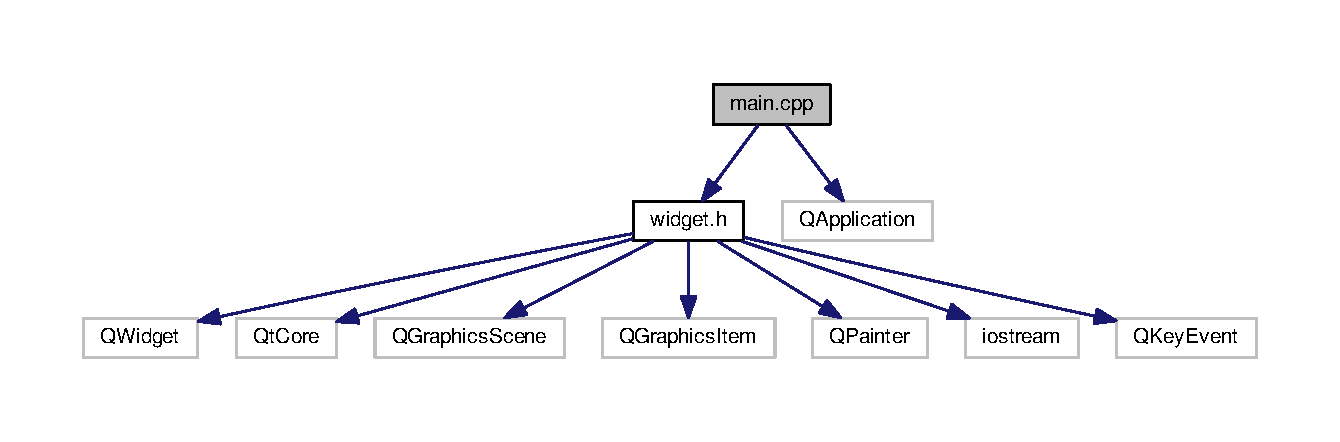
\includegraphics[width=350pt]{main_8cpp__incl}
\end{center}
\end{figure}
\subsection*{Functions}
\begin{DoxyCompactItemize}
\item 
int \hyperlink{main_8cpp_a0ddf1224851353fc92bfbff6f499fa97}{main} (int argc, char $\ast$argv\mbox{[}$\,$\mbox{]})
\end{DoxyCompactItemize}


\subsection{Function Documentation}
\index{main.\+cpp@{main.\+cpp}!main@{main}}
\index{main@{main}!main.\+cpp@{main.\+cpp}}
\subsubsection[{\texorpdfstring{main(int argc, char $\ast$argv[])}{main(int argc, char *argv[])}}]{\setlength{\rightskip}{0pt plus 5cm}int main (
\begin{DoxyParamCaption}
\item[{int}]{argc, }
\item[{char $\ast$}]{argv\mbox{[}$\,$\mbox{]}}
\end{DoxyParamCaption}
)}\hypertarget{main_8cpp_a0ddf1224851353fc92bfbff6f499fa97}{}\label{main_8cpp_a0ddf1224851353fc92bfbff6f499fa97}

\hypertarget{myitem_8cpp}{}\section{Tako/myitem.cpp File Reference}
\label{myitem_8cpp}\index{Tako/myitem.\+cpp@{Tako/myitem.\+cpp}}
{\ttfamily \#include \char`\"{}myitem.\+h\char`\"{}}\\*
Include dependency graph for myitem.\+cpp\+:
\nopagebreak
\begin{figure}[H]
\begin{center}
\leavevmode
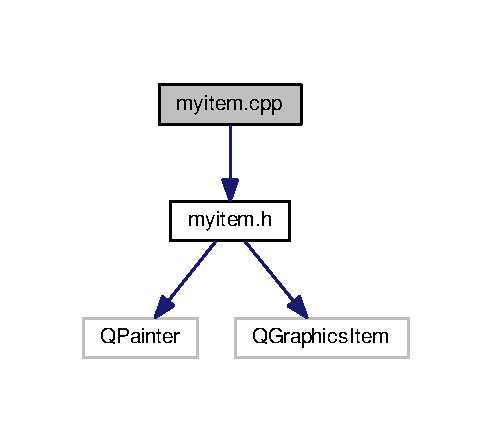
\includegraphics[width=236pt]{myitem_8cpp__incl}
\end{center}
\end{figure}

\hypertarget{myitem_8h}{}\section{myitem.\+h File Reference}
\label{myitem_8h}\index{myitem.\+h@{myitem.\+h}}
{\ttfamily \#include $<$Q\+Painter$>$}\\*
{\ttfamily \#include $<$Q\+Graphics\+Item$>$}\\*
Include dependency graph for myitem.\+h\+:\nopagebreak
\begin{figure}[H]
\begin{center}
\leavevmode
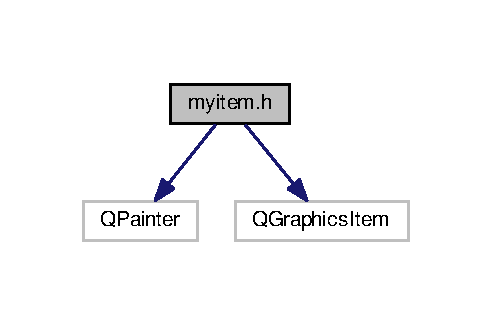
\includegraphics[width=236pt]{myitem_8h__incl}
\end{center}
\end{figure}
This graph shows which files directly or indirectly include this file\+:\nopagebreak
\begin{figure}[H]
\begin{center}
\leavevmode
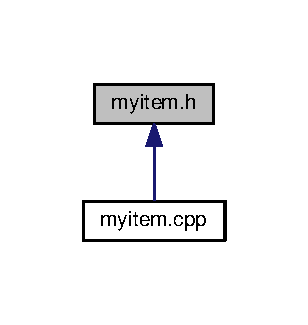
\includegraphics[width=148pt]{myitem_8h__dep__incl}
\end{center}
\end{figure}
\subsection*{Classes}
\begin{DoxyCompactItemize}
\item 
class \hyperlink{class_my_item}{My\+Item}
\end{DoxyCompactItemize}

\hypertarget{widget_8cpp}{}\section{widget.\+cpp File Reference}
\label{widget_8cpp}\index{widget.\+cpp@{widget.\+cpp}}
{\ttfamily \#include \char`\"{}widget.\+h\char`\"{}}\\*
{\ttfamily \#include \char`\"{}ui\+\_\+widget.\+h\char`\"{}}\\*
Include dependency graph for widget.\+cpp\+:\nopagebreak
\begin{figure}[H]
\begin{center}
\leavevmode
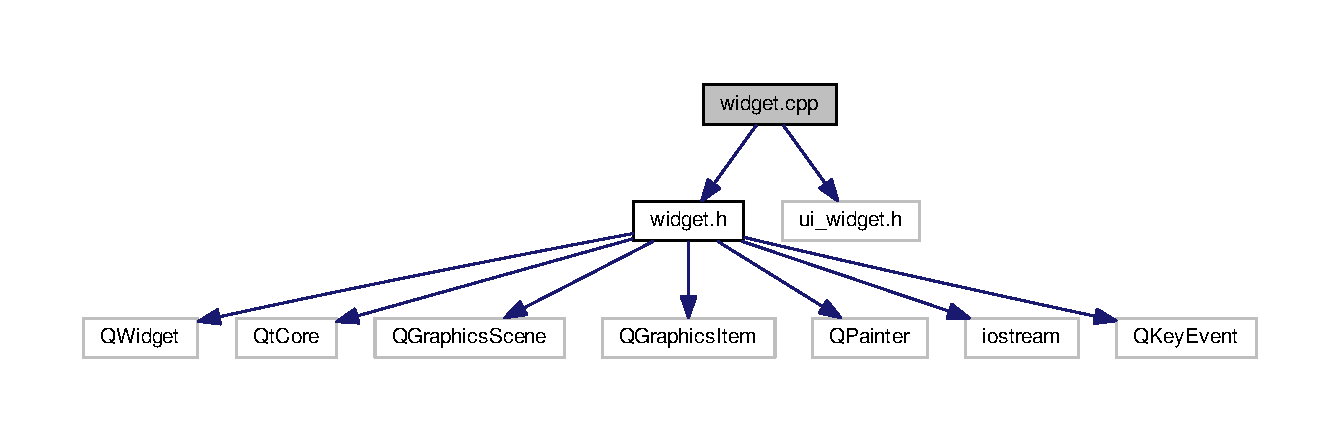
\includegraphics[width=350pt]{widget_8cpp__incl}
\end{center}
\end{figure}
\subsection*{Variables}
\begin{DoxyCompactItemize}
\item 
int \hyperlink{widget_8cpp_ac9b5a410a1af8bfcb0b5aa289ee96bfa}{game\+\_\+score}
\item 
\hyperlink{class_my_item}{My\+Item} $\ast$ \hyperlink{widget_8cpp_a29c8d9815e2b7de236eec8edc926cc10}{Act}
\end{DoxyCompactItemize}


\subsection{Variable Documentation}
\index{widget.\+cpp@{widget.\+cpp}!Act@{Act}}
\index{Act@{Act}!widget.\+cpp@{widget.\+cpp}}
\subsubsection[{\texorpdfstring{Act}{Act}}]{\setlength{\rightskip}{0pt plus 5cm}{\bf My\+Item}$\ast$ Act}\hypertarget{widget_8cpp_a29c8d9815e2b7de236eec8edc926cc10}{}\label{widget_8cpp_a29c8d9815e2b7de236eec8edc926cc10}


Definition at line 4 of file widget.\+cpp.

\index{widget.\+cpp@{widget.\+cpp}!game\+\_\+score@{game\+\_\+score}}
\index{game\+\_\+score@{game\+\_\+score}!widget.\+cpp@{widget.\+cpp}}
\subsubsection[{\texorpdfstring{game\+\_\+score}{game_score}}]{\setlength{\rightskip}{0pt plus 5cm}int game\+\_\+score}\hypertarget{widget_8cpp_ac9b5a410a1af8bfcb0b5aa289ee96bfa}{}\label{widget_8cpp_ac9b5a410a1af8bfcb0b5aa289ee96bfa}


Definition at line 3 of file widget.\+cpp.


\hypertarget{widget_8h}{}\section{widget.\+h File Reference}
\label{widget_8h}\index{widget.\+h@{widget.\+h}}
{\ttfamily \#include $<$Q\+Widget$>$}\\*
{\ttfamily \#include $<$Qt\+Core$>$}\\*
{\ttfamily \#include $<$Q\+Graphics\+Scene$>$}\\*
{\ttfamily \#include $<$Q\+Graphics\+Item$>$}\\*
{\ttfamily \#include $<$Q\+Painter$>$}\\*
{\ttfamily \#include $<$iostream$>$}\\*
{\ttfamily \#include $<$Q\+Key\+Event$>$}\\*
Include dependency graph for widget.\+h\+:\nopagebreak
\begin{figure}[H]
\begin{center}
\leavevmode
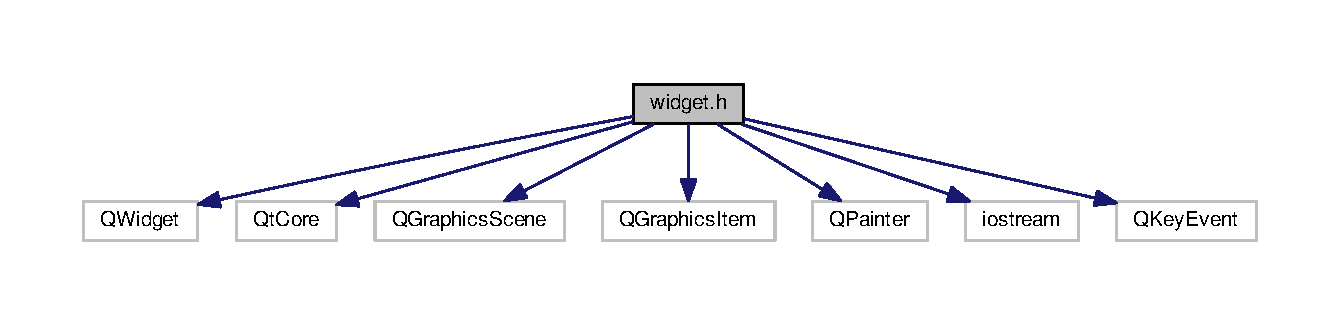
\includegraphics[width=350pt]{widget_8h__incl}
\end{center}
\end{figure}
This graph shows which files directly or indirectly include this file\+:\nopagebreak
\begin{figure}[H]
\begin{center}
\leavevmode
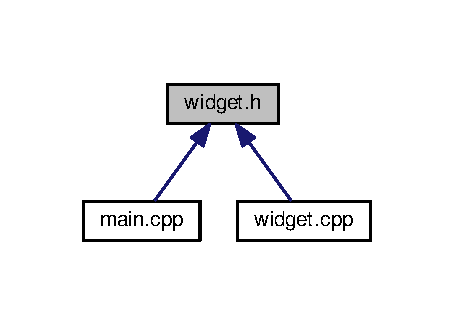
\includegraphics[width=218pt]{widget_8h__dep__incl}
\end{center}
\end{figure}
\subsection*{Classes}
\begin{DoxyCompactItemize}
\item 
class \hyperlink{class_widget}{Widget}
\item 
class \hyperlink{class_my_item}{My\+Item}
\end{DoxyCompactItemize}
\subsection*{Namespaces}
\begin{DoxyCompactItemize}
\item 
 \hyperlink{namespace_ui}{Ui}
\end{DoxyCompactItemize}
\subsection*{Macros}
\begin{DoxyCompactItemize}
\item 
\#define \hyperlink{widget_8h_a45ba202b05caf39795aeca91b0ae547e}{T\+I\+M\+E\+O\+UT}~30
\item 
\#define \hyperlink{widget_8h_a8d23feea868a983c8c2b661e1e16972f}{R\+ED}~0
\item 
\#define \hyperlink{widget_8h_ac916275bd93e31ae604687be03e98896}{G\+RE}~1
\end{DoxyCompactItemize}


\subsection{Macro Definition Documentation}
\index{widget.\+h@{widget.\+h}!G\+RE@{G\+RE}}
\index{G\+RE@{G\+RE}!widget.\+h@{widget.\+h}}
\subsubsection[{\texorpdfstring{G\+RE}{GRE}}]{\setlength{\rightskip}{0pt plus 5cm}\#define G\+RE~1}\hypertarget{widget_8h_ac916275bd93e31ae604687be03e98896}{}\label{widget_8h_ac916275bd93e31ae604687be03e98896}


Definition at line 13 of file widget.\+h.

\index{widget.\+h@{widget.\+h}!R\+ED@{R\+ED}}
\index{R\+ED@{R\+ED}!widget.\+h@{widget.\+h}}
\subsubsection[{\texorpdfstring{R\+ED}{RED}}]{\setlength{\rightskip}{0pt plus 5cm}\#define R\+ED~0}\hypertarget{widget_8h_a8d23feea868a983c8c2b661e1e16972f}{}\label{widget_8h_a8d23feea868a983c8c2b661e1e16972f}


Definition at line 12 of file widget.\+h.

\index{widget.\+h@{widget.\+h}!T\+I\+M\+E\+O\+UT@{T\+I\+M\+E\+O\+UT}}
\index{T\+I\+M\+E\+O\+UT@{T\+I\+M\+E\+O\+UT}!widget.\+h@{widget.\+h}}
\subsubsection[{\texorpdfstring{T\+I\+M\+E\+O\+UT}{TIMEOUT}}]{\setlength{\rightskip}{0pt plus 5cm}\#define T\+I\+M\+E\+O\+UT~30}\hypertarget{widget_8h_a45ba202b05caf39795aeca91b0ae547e}{}\label{widget_8h_a45ba202b05caf39795aeca91b0ae547e}


Definition at line 11 of file widget.\+h.


%--- End generated contents ---

% Index
\backmatter
\newpage
\phantomsection
\clearemptydoublepage
\addcontentsline{toc}{chapter}{Index}
\printindex

\end{document}
